\documentclass[11pt]{article}
\usepackage[utf8]{inputenc}
\usepackage[russian]{babel}
\usepackage[T1]{fontenc}
\usepackage{amssymb,amsmath,clrscode,graphicx,indentfirst}

\author{Олег Смирнов}
\title{Курс kiev-clrs -- Лекция 4. Сортировка quicksort, рандомизированные алгоритмы}
\date{3 апреля 2009 г.}

\begin{document}
\maketitle
\tableofcontents

\newpage
\setlength{\parskip}{1ex plus 0.5ex minus 0.2ex}
\section{Цель лекции}
\begin{itemize}
\item 
\end{itemize}

\section{Алгоритм Хора: quicksort}

Алгоритм входит в Top10 вместе с методом Монте-Карло, симплекс-методом и быстрым преобразованием Фурье.

Алгоритм вида "Разделяй и властвуй", сортировка делается "на месте", так же как сортировка вставкой в отличии от сортировки слиянием. Шаги алгоритма:

\begin{itemize}
\item Divide: деление массива на два подмассива относительно опорного элемента (pivot) $x$: элементы левого подмассива $\leqslant x$, правого $\geqslant x$
\item Conquer: рекурсивная сортировка двух подмассивов
\item Combine: тривиально
\end{itemize}
Проще говоря, quicksort -- это рекурсивное деление, тогда как mergesort -- рекурсивное слияние.

Ключевой частью алгоритма является процедуры Partition, которая выполняется за линейное время $(O(n))$:

\begin{codebox}
\Procname{$\proc{Partition}(A, p, q)$ \Comment $A[p \twodots q]$}
\li	$x \gets A[p]$	\Comment pivot
\li	$i \gets p$
\li	\For $j \gets p+1$ \To $q$
\li		\Do \If $A[j] \leqslant x$
\li		\Then $i \gets i+1$
\li			exchange $A[i] \iff A[j]$
		\End
	\End
\li	exchange $A[p] \iff A[j]$
\li \Return i
\End
\end{codebox}

\begin{figure}[ht]
  \centering
  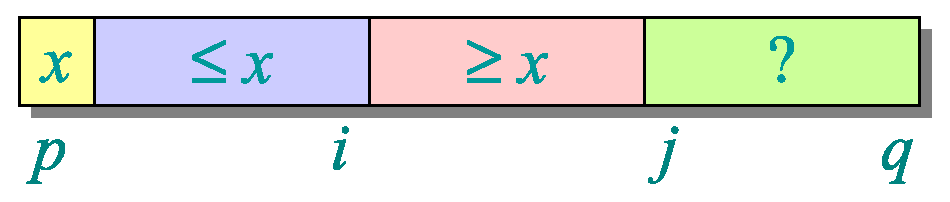
\includegraphics[width=3in]{lecture4/invariant.eps}
  \caption{Инвариант цикла}
  \label{fig:invariant}
\end{figure}

Доказательство инварианта (рис. \ref{fig:invariant}):
\nopagebreak
\begin{itemize}
\item Инициализация: в начале цикла инвариант выполняется, так как $i = p$ и $j = p+1$ 
\item Сохранение: если на очередном шаге $A[j] \geqslant x$, инвариант выполняется и счетчик $j$ увеличивается на единицу
\item Завершение: если $A[j] \leqslant x$, инвариант выполняется через обмен элемента $A[j]$ с $A[i]$ и сдвига границы левой части массива $i = i+1$
\end{itemize}

Алгоритм весьма прост для понимания. Время выполнения процедуры равно $O(n)$ для массива из $n$ элементов.

\begin{figure}[ht]
  \centering
  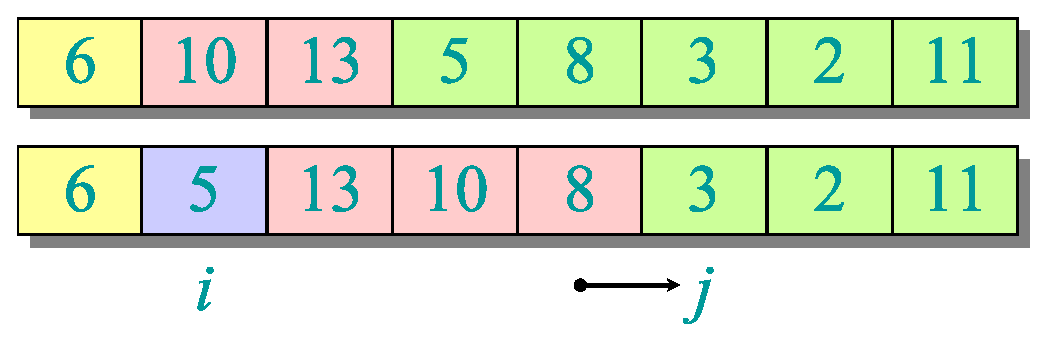
\includegraphics[width=3in]{lecture4/example1.eps}
  \caption{Пример работы}
  \label{fig:example1}
\end{figure}

Пример работы процедуры (рис. \ref{fig:example1}):
\begin{itemize}
\item шаге 0: $i$ на $6$, $j$ на $10$
\item шаге 1: обменеваются местами $10$ и $5$, $j$ на $8$
\item шаге 2: обменеваются $13$ и $3$, $i$ на $3$, $j$ на $2$
\item шаге 2: обменеваются $10$ и $2$, $i$ на $2$, $j$ на $11$
\item на последнем шаге опорный элемент перемещается на середину (вместо $2$) 
\end{itemize}
В конце работы элементы меньше или равные опорному находятся слева, остальные -- справа.

Алгоритм QuickSort:
\nopagebreak
\begin{codebox}
\Procname{$\proc{Quicksort}(A, p, q)$}
\li	\If $p < q$
\li		\Then $r \gets $ Partition(A, p, q)
\li			Quicksort(A, p, r-1)
\li			Quicksort(A, r+1, q)
	\End
\End
\end{codebox}

Начальные параметры вызова: Quicksort(A, 1, n)

Один из способов оптимизации Quicksort -- использования отдельной процедуры для маленьких массивов, например для $n \leqslant 5$ (например прямое сравнение). Также применяют хвостовую оптимизацию рекурсии.

\section{Анализ quicksort}

Предположим, что все элементы различны, т.к. в случае дублирующихся элементов алгоритм работает более эффективно.

\subsection{Наихудший случай}

Легко видеть, что наихудшим образом алгоритм будет себя вести, если подпрограмма, выполняющая разбиение, порождает одну подзадачу с $n-1$ элементов, а вторую -- с $0$ элементов. Это происходит в том случае, если все элементы массива больше либо меньше выбранного опорного элемента.

\begin{align*}
  T(n) = \\
    = T(0) + T(n-1) + \Theta(n) \\ 
    = \Theta(1) + T(n-1) + \Theta(n) \\
    = T(n-1) + \Theta(n) \\
    = \Theta(n^2) \text{ (арифметическая прогрессия)}
\end{align*}

Дерево рекурсии для случая $T(n) = T(0) + T(n-1) + cn$ (рис. \ref{fig:tree1}). 

\begin{figure}[ht]
  \centering
  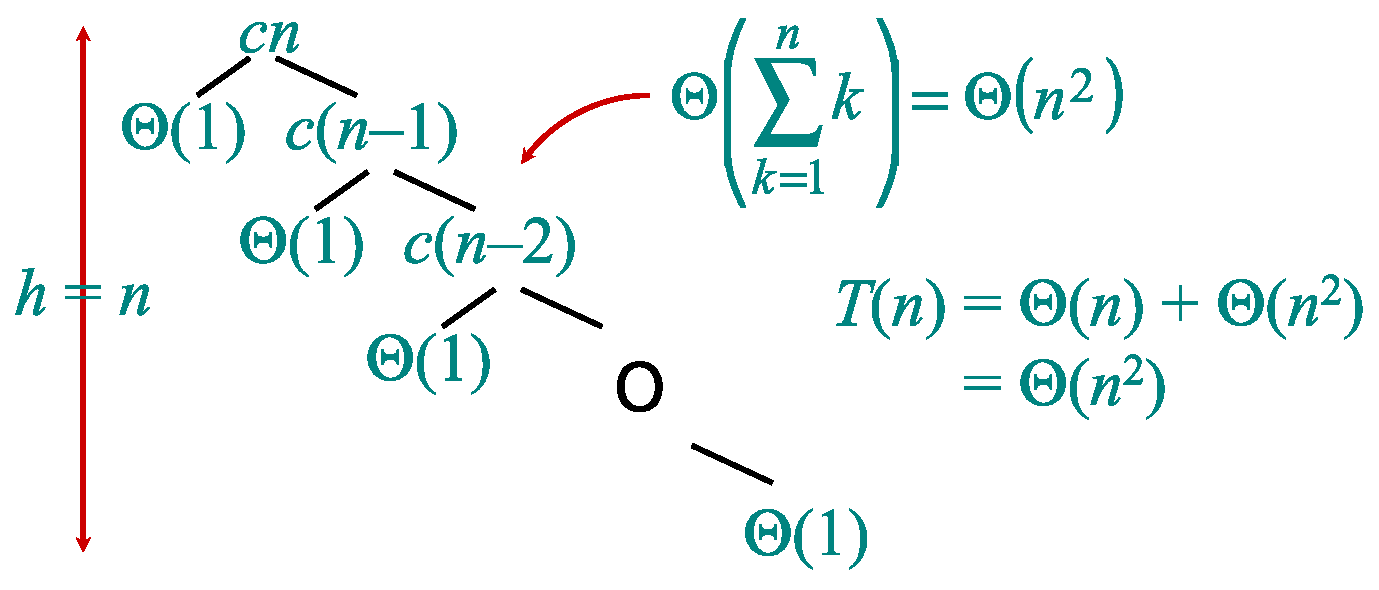
\includegraphics[width=3in]{lecture4/tree1.eps}
  \caption{Дерево наихудшего случая}
  \label{fig:tree1}
\end{figure}

Высота дерева $h = n$. Сумма правой ветви -- $\Theta(\sum_{k=1}ck) = \Theta(n^2)$, левых ветвей -- ${\Theta(1)}n$. Суммарное время работы в таком случае равно $T(n) = \Theta(n) + \Theta(n^2) = \Theta(n^2)$

\subsection{Наилучший случай}

Возникает, когда процедура делит массив на две равные части: $n/2$ и $n/2$

Время работы оценивается рекуррентностью: $T(n) \leqslant 2T(n/2) + \Theta(n)$

Согласно второму случае основного метода, ответ $T(n) = O(n \lg n)$

\subsection{Средний случай}

\section{Рандомизированный quicksort}

\section{Анализ рандомизированного quicksort}

\subsection{Наихудший случай}

\end{document}
